% Asset ID: AS1VectorsTikZ-002
% Asset type: TikZ diagram
% Suggested file: tikz/AS1VectorsTikZ-002_magnitude_direction.tex
% Source: CCEA AS1-VEC-LO002; Phase 1 Core Theory 2 and 3
% Related lesson section: Magnitude and direction of a vector
% Purpose: Show magnitude and direction of a 2D vector using a right-angled triangle.
% Boundary note: 2D vectors only.

\documentclass[tikz,border=8pt]{standalone}
\usepackage{amsmath}
\usetikzlibrary{arrows.meta, angles, quotes}
\begin{document}
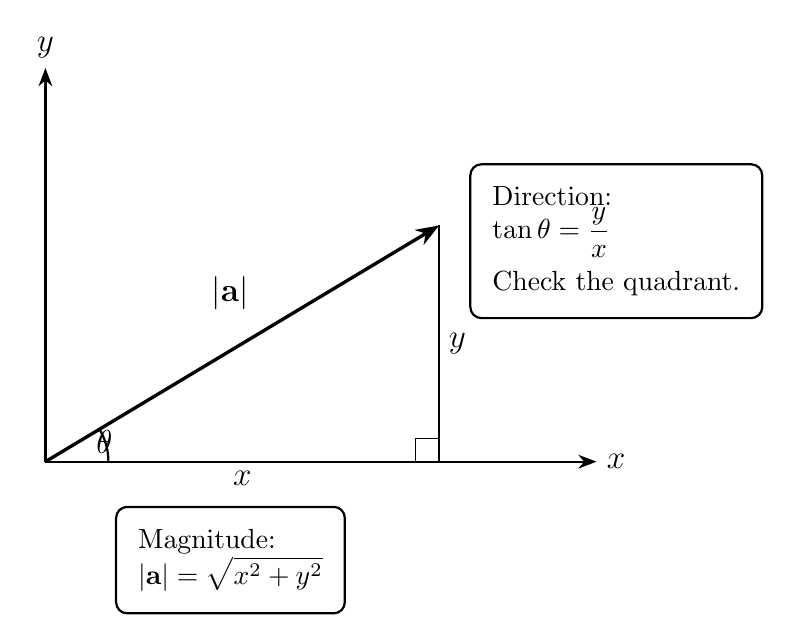
\begin{tikzpicture}[>=Stealth,axis/.style={->, thick},vector/.style={->, very thick},side/.style={thick},label/.style={font=\large},formula/.style={draw, rounded corners, thick, align=left, inner sep=8pt}]
\draw[axis] (0,0) -- (7,0) node[right,label] {$x$};
\draw[axis] (0,0) -- (0,5) node[above,label] {$y$};
\coordinate (O) at (0,0); \coordinate (X) at (5,0); \coordinate (P) at (5,3);
\draw[side] (O) -- (X); \draw[side] (X) -- (P); \draw[vector] (O) -- (P);
\draw (4.7,0) -- (4.7,0.3) -- (5,0.3);
\node[label,below] at (2.5,0) {$x$}; \node[label,right] at (5,1.5) {$y$}; \node[label,above left] at (2.7,1.8) {$|\mathbf{a}|$}; \node[label] at (0.75,0.25) {$\theta$};
\draw[thick] (0.8,0) arc[start angle=0,end angle=31,radius=0.8];
\node[formula] at (2.35,-1.25) {Magnitude:\\ $\displaystyle |\mathbf{a}|=\sqrt{x^2+y^2}$};
\node[formula] at (7.25,2.8) {Direction:\\ $\displaystyle \tan\theta=\frac{y}{x}$\\[4pt] Check the quadrant.};
\end{tikzpicture}
\end{document}
